% ============================================================
%  Soutenance – Moteur de Recherche Sémantique (pgvector)
%  Bases de Données Avancées – ESI Alger – 2CS SIQ1
%  Juin 2026
% ============================================================

\documentclass[aspectratio=169, 10pt]{beamer}
\usepackage[T1]{fontenc}
\usepackage[utf8]{inputenc}
\usepackage{beamerthemeASTRA}

% ---- Packages ----
\usepackage{amsmath, amssymb}
\usepackage{booktabs}
\usepackage{multicol}
\usepackage{caption}
\usepackage{hyperref}
\usepackage{array}
\usepackage{pifont}
\usepackage{ragged2e}
\usepackage{tikz}
\usetikzlibrary{arrows.meta, positioning, shapes.geometric, fit, calc}

% ---- Couleurs TikZ (du rapport) ----
\definecolor{tikzblue}{HTML}{2563EB}
\definecolor{tikzgreen}{HTML}{059669}
\definecolor{tikzorange}{HTML}{D97706}
\definecolor{tikzred}{HTML}{DC2626}
\definecolor{tikzpurple}{HTML}{7C3AED}
\definecolor{tikzgray}{HTML}{6B7280}
\definecolor{tikzlightblue}{HTML}{DBEAFE}
\definecolor{tikzlightgreen}{HTML}{D1FAE5}
\definecolor{tikzlightorange}{HTML}{FEF3C7}
\definecolor{tikzlightred}{HTML}{FEE2E2}
\definecolor{tikzlightpurple}{HTML}{EDE9FE}

% ---- Hyperlinks ----
\hypersetup{
  colorlinks = true,
  urlcolor   = ASTRAaccent,
  linkcolor  = ASTRAblue,
  citecolor  = ASTRAblue
}

% ============================================================
%  METADATA
% ============================================================
\title{Conception et Impl\'{e}mentation d'un\\Moteur de Recherche S\'{e}mantique\\
\normalsize Bas\'{e} sur PostgreSQL + pgvector}

\author{%
  \textbf{\textcolor{ASTRAnavy}{Idriss Yacine ZIADI}}\textcolor{ASTRAnavy}{,~}%
  \textbf{\textcolor{ASTRAnavy}{Rayan BOUKAKIOU}}%
}

\setAffiliations{%
  \'{E}cole nationale Sup\'{e}rieure d'Informatique (ESI) -- Alger\\
  2CS SIQ1 -- Bases de Donn\'{e}es Avanc\'{e}es -- Ann\'{e}e 2025--2026%
}

\setCorrespondingAuthor{%
  Encadr\'{e} par : \textbf{Mme AMROUCHE Karima}%
}

\setPaperID{Mini-projet BDA}

\date{Juin 2026}

% ============================================================
\begin{document}
% ============================================================

% ------------------------------------------------------------
%  SLIDE 1 – Page de titre
% ------------------------------------------------------------
\begin{frame}[plain]
  \titlepage
\end{frame}

% ------------------------------------------------------------
%  SLIDE 2 – Plan
% ------------------------------------------------------------
\begin{frame}{Plan}
  \begin{columns}[T]
    \begin{column}{0.55\textwidth}
      \setbeamerfont{enumerate item}{size=\large}
      \begin{enumerate}
        \setlength{\itemsep}{0.8em}
        \item {\large Probl\'{e}matique}
        \item {\large Architecture \& M\'{e}thodologie}
        \item {\large Impl\'{e}mentation}
        \item {\large R\'{e}sultats}
        \item {\large Conclusion}
        \item {\large R\'{e}f\'{e}rences}
      \end{enumerate}
    \end{column}
    \begin{column}{0.42\textwidth}
      \begin{block}{En bref}
        \begin{itemize}
          \item 1\,964 documents (AG News)
          \item Embeddings 384 dimensions
          \item Precision@5 : \textbf{0.81}
          \item Temps de r\'{e}ponse : \textbf{19.8\,ms}
        \end{itemize}
      \end{block}
    \end{column}
  \end{columns}
\end{frame}

% ------------------------------------------------------------
%  SLIDE 3 – Problématique
% ------------------------------------------------------------
\begin{frame}{Probl\'{e}matique}
  \begin{columns}[T]
    \begin{column}{0.52\textwidth}
      \begin{block}{Recherche lexicale (TF-IDF)}
        \begin{itemize}
          \item Correspondance \textbf{exacte} de mots-cl\'{e}s
          \item ``automobile'' $\neq$ ``voiture''
          \item Ignore synonymie et paraphrase
          \item Rapide mais limit\'{e}e en pertinence
        \end{itemize}
      \end{block}
      \vspace{0.5em}
      \begin{block}{Recherche s\'{e}mantique}
        \begin{itemize}
          \item Recherche par le \textbf{sens} du texte
          \item ``automobile'' $\approx$ ``voiture'' $\approx$ ``v\'{e}hicule''
          \item Capture les relations s\'{e}mantiques
          \item Meilleure pertinence
        \end{itemize}
      \end{block}
    \end{column}
    \begin{column}{0.45\textwidth}
      \begin{block}{Similarit\'{e} cosinus}
        \centering
        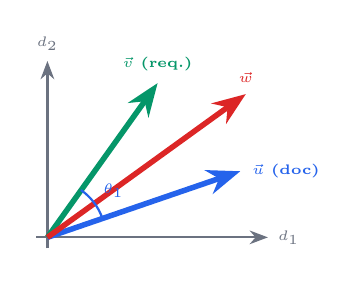
\begin{tikzpicture}[>=Stealth, scale=0.7]
          \draw[->, thick, tikzgray] (-0.2,0) -- (4,0) node[right, font=\tiny] {$d_1$};
          \draw[->, thick, tikzgray] (0,-0.2) -- (0,3.2) node[above, font=\tiny] {$d_2$};
          \draw[->, line width=2pt, tikzblue] (0,0) -- (3.5,1.2) node[right, font=\tiny\bfseries] {$\vec{u}$ (doc)};
          \draw[->, line width=2pt, tikzgreen] (0,0) -- (2,2.8) node[above, font=\tiny\bfseries] {$\vec{v}$ (req.)};
          \draw[->, line width=2pt, tikzred] (0,0) -- (3.6,2.6) node[above, font=\tiny\bfseries] {$\vec{w}$};
          \draw[tikzblue, thick] (1,0.34) arc[start angle=19, end angle=55, radius=1.05];
          \node[tikzblue, font=\tiny\bfseries] at (1.2,0.85) {$\theta_1$};
        \end{tikzpicture}
      \end{block}
      \vspace{0.3em}
      \textbf{\textcolor{ASTRAorange}{Question :}}
      \textit{\small Comment impl\'{e}menter une recherche s\'{e}mantique performante avec des technologies open-source ?}
    \end{column}
  \end{columns}
\end{frame}

% ------------------------------------------------------------
%  SLIDE 4 – Architecture
% ------------------------------------------------------------
\begin{frame}{Architecture du syst\`{e}me}
  \centering
  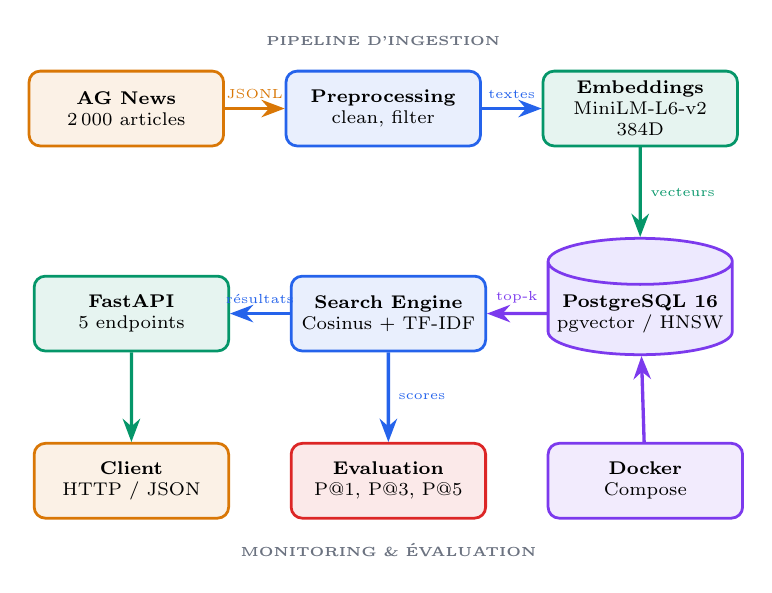
\begin{tikzpicture}[
      node distance=0.4cm and 0.6cm,
      component/.style={draw=#1, fill=#1!10, rounded corners=4pt, minimum width=2.6cm, minimum height=1cm, align=center, font=\scriptsize, line width=1pt},
      db/.style={draw=tikzpurple, fill=tikzlightpurple, cylinder, shape border rotate=90, aspect=0.25, minimum width=2.2cm, minimum height=1.1cm, align=center, font=\scriptsize, line width=1pt},
      dataflow/.style={->, >=Stealth, line width=1.2pt, color=tikzgray},
      grouplabel/.style={font=\tiny\bfseries, color=tikzgray},
      >=Stealth, scale=0.95, every node/.style={transform shape}
  ]
    \node[component=tikzorange] (datasrc) at (0,0) {\textbf{AG News}\\2\,000 articles};
    \node[component=tikzblue, right=0.8cm of datasrc] (preproc) {\textbf{Preprocessing}\\clean, filter};
    \node[component=tikzgreen, right=0.8cm of preproc] (embed) {\textbf{Embeddings}\\MiniLM-L6-v2\\384D};
    \node[db, below=1.2cm of embed] (db) {\textbf{PostgreSQL 16}\\pgvector / HNSW};
    \node[component=tikzblue, left=0.8cm of db] (search) {\textbf{Search Engine}\\Cosinus + TF-IDF};
    \node[component=tikzgreen, left=0.8cm of search] (api) {\textbf{FastAPI}\\5 endpoints};
    \node[component=tikzred, below=1.2cm of search] (eval) {\textbf{Evaluation}\\P@1, P@3, P@5};
    \node[component=tikzorange, left=0.8cm of eval] (client) {\textbf{Client}\\HTTP / JSON};
    \node[component=tikzpurple, right=0.8cm of eval] (docker) {\textbf{Docker}\\Compose};

    \draw[dataflow, tikzorange] (datasrc) -- node[above, font=\tiny] {JSONL} (preproc);
    \draw[dataflow, tikzblue] (preproc) -- node[above, font=\tiny] {textes} (embed);
    \draw[dataflow, tikzgreen] (embed) -- node[right, font=\tiny] {vecteurs} (db);
    \draw[dataflow, tikzpurple] (db) -- node[above, font=\tiny] {top-k} (search);
    \draw[dataflow, tikzblue] (search) -- node[above, font=\tiny] {r\'{e}sultats} (api);
    \draw[dataflow, tikzblue] (search) -- node[right, font=\tiny] {scores} (eval);
    \draw[dataflow, tikzgreen] (api) -- (client);
    \draw[dataflow, tikzpurple] (docker) -- (db);

    \node[grouplabel, above=0.2cm of preproc] {PIPELINE D'INGESTION};
    \node[grouplabel, below=0.2cm of eval] {MONITORING \& \'{E}VALUATION};
  \end{tikzpicture}
\end{frame}

% ------------------------------------------------------------
%  SLIDE 5 – Pipeline
% ------------------------------------------------------------
\begin{frame}{Pipeline de traitement}
  \centering
  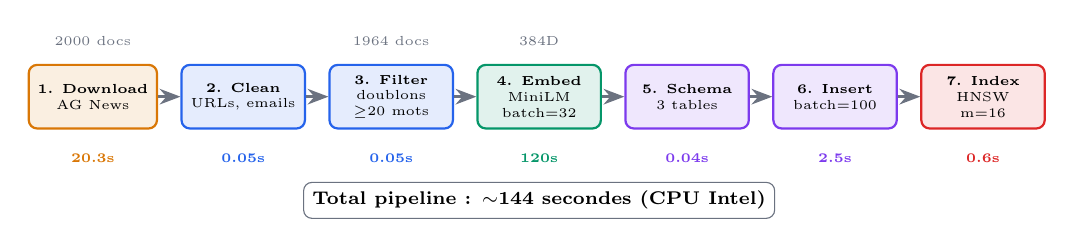
\begin{tikzpicture}[
      node distance=0.05cm,
      step/.style={draw=#1, fill=#1!12, rounded corners=3pt, minimum width=1.65cm, minimum height=0.85cm, align=center, font=\tiny, line width=0.8pt},
      timelab/.style={font=\tiny\bfseries, color=#1},
      arrow/.style={->, >=Stealth, line width=1pt, tikzgray},
      scale=0.95, every node/.style={transform shape}
  ]
    \node[step=tikzorange] (s1) at (0,0) {\textbf{1. Download}\\AG News};
    \node[step=tikzblue, right=0.3cm of s1] (s2) {\textbf{2. Clean}\\URLs, emails};
    \node[step=tikzblue, right=0.3cm of s2] (s3) {\textbf{3. Filter}\\doublons\\$\geq$20 mots};
    \node[step=tikzgreen, right=0.3cm of s3] (s4) {\textbf{4. Embed}\\MiniLM\\batch=32};
    \node[step=tikzpurple, right=0.3cm of s4] (s5) {\textbf{5. Schema}\\3 tables};
    \node[step=tikzpurple, right=0.3cm of s5] (s6) {\textbf{6. Insert}\\batch=100};
    \node[step=tikzred, right=0.3cm of s6] (s7) {\textbf{7. Index}\\HNSW\\m=16};

    \draw[arrow] (s1) -- (s2);
    \draw[arrow] (s2) -- (s3);
    \draw[arrow] (s3) -- (s4);
    \draw[arrow] (s4) -- (s5);
    \draw[arrow] (s5) -- (s6);
    \draw[arrow] (s6) -- (s7);

    \node[timelab=tikzorange, below=0.2cm of s1] {20.3s};
    \node[timelab=tikzblue, below=0.2cm of s2] {0.05s};
    \node[timelab=tikzblue, below=0.2cm of s3] {0.05s};
    \node[timelab=tikzgreen, below=0.2cm of s4] {120s};
    \node[timelab=tikzpurple, below=0.2cm of s5] {0.04s};
    \node[timelab=tikzpurple, below=0.2cm of s6] {2.5s};
    \node[timelab=tikzred, below=0.2cm of s7] {0.6s};

    \node[font=\tiny, tikzgray, above=0.12cm of s1] {2000 docs};
    \node[font=\tiny, tikzgray, above=0.12cm of s3] {1964 docs};
    \node[font=\tiny, tikzgray, above=0.12cm of s4] {384D};

    \node[draw=tikzgray, rounded corners=3pt, fill=white, font=\scriptsize\bfseries, below=0.7cm of s4] {Total pipeline : $\sim$144 secondes (CPU Intel)};
  \end{tikzpicture}

  \vspace{1em}
  \begin{columns}[T]
    \begin{column}{0.48\textwidth}
      \begin{block}{Mod\`{e}le d'embeddings}
        \begin{itemize}
          \item \textbf{all-MiniLM-L6-v2} (Sentence-Transformers)
          \item 384 dimensions, 22.7M param\`{e}tres
          \item Score STS Benchmark : 0.8282
        \end{itemize}
      \end{block}
    \end{column}
    \begin{column}{0.48\textwidth}
      \begin{block}{Index HNSW}
        \begin{itemize}
          \item $m=16$ (connexions par n\oe ud)
          \item $ef\_construction=64$
          \item Recall quasi-parfait, construction 0.6s
        \end{itemize}
      \end{block}
    \end{column}
  \end{columns}
\end{frame}

% ------------------------------------------------------------
%  SLIDE 6 – Implémentation
% ------------------------------------------------------------
\begin{frame}{Impl\'{e}mentation}
  \begin{columns}[T]
    \begin{column}{0.45\textwidth}
      \begin{block}{Sch\'{e}ma de la base (3 tables)}
        \centering
        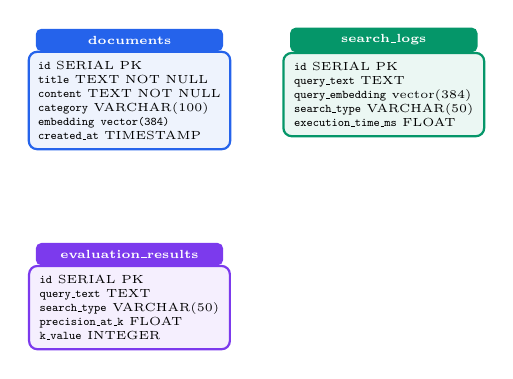
\begin{tikzpicture}[
            entity/.style={draw=#1, fill=#1!8, rounded corners=3pt, minimum width=3cm, align=left, font=\tiny, line width=0.8pt, inner sep=4pt},
            entitytitle/.style={font=\tiny\bfseries, text=white, fill=#1, rounded corners=2pt, minimum width=2.8cm, align=center, inner sep=3pt},
            scale=0.85, every node/.style={transform shape}
        ]
          \node[entitytitle=tikzblue] (dt) at (0,0) {documents};
          \node[entity=tikzblue, below=-0.3pt of dt, anchor=north] (d) {
              \texttt{id} SERIAL PK\\
              \texttt{title} TEXT NOT NULL\\
              \texttt{content} TEXT NOT NULL\\
              \texttt{category} VARCHAR(100)\\
              \texttt{\textbf{embedding vector(384)}}\\
              \texttt{created\_at} TIMESTAMP
          };

          \node[entitytitle=tikzgreen] (lt) at (3.8,0) {search\_logs};
          \node[entity=tikzgreen, below=-0.3pt of lt, anchor=north] (l) {
              \texttt{id} SERIAL PK\\
              \texttt{query\_text} TEXT\\
              \texttt{query\_embedding} vector(384)\\
              \texttt{search\_type} VARCHAR(50)\\
              \texttt{execution\_time\_ms} FLOAT
          };

          \node[entitytitle=tikzpurple] (et) at (0,-3.2) {evaluation\_results};
          \node[entity=tikzpurple, below=-0.3pt of et, anchor=north] (e) {
              \texttt{id} SERIAL PK\\
              \texttt{query\_text} TEXT\\
              \texttt{search\_type} VARCHAR(50)\\
              \texttt{precision\_at\_k} FLOAT\\
              \texttt{k\_value} INTEGER
          };
        \end{tikzpicture}
      \end{block}
    \end{column}
    \begin{column}{0.52\textwidth}
      \begin{block}{API REST (FastAPI)}
        \footnotesize
        \begin{tabular}{@{}lll@{}}
          \toprule
          \textbf{M\'{e}thode} & \textbf{Endpoint} & \textbf{Description} \\
          \midrule
          GET  & \texttt{/health}          & \'{E}tat de sant\'{e} \\
          POST & \texttt{/search/semantic} & Recherche s\'{e}mantique \\
          POST & \texttt{/search/lexical}  & Recherche TF-IDF \\
          POST & \texttt{/search/compare}  & Comparaison \\
          GET  & \texttt{/stats}           & Statistiques \\
          \bottomrule
        \end{tabular}
      \end{block}
      \vspace{0.5em}
      \begin{block}{Infrastructure Docker}
        \centering
        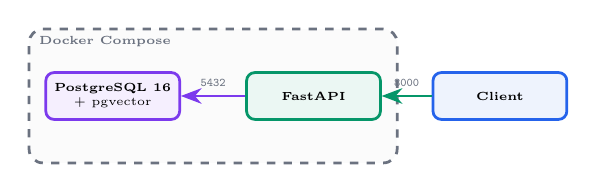
\begin{tikzpicture}[
            container/.style={draw=#1, fill=#1!8, rounded corners=3pt, minimum width=2cm, minimum height=0.7cm, align=center, font=\tiny, line width=1pt},
            >=Stealth, scale=0.85, every node/.style={transform shape}
        ]
          \node[draw=tikzgray, dashed, fill=gray!3, rounded corners=5pt, minimum width=5.5cm, minimum height=2cm, line width=1pt] (host) at (1.5,0) {};
          \node[font=\tiny\bfseries, tikzgray, anchor=north west] at (host.north west) {\,Docker Compose};
          \node[container=tikzpurple] (pg) at (0,0) {\textbf{PostgreSQL 16}\\+ pgvector};
          \node[container=tikzgreen] (api) at (3,0) {\textbf{FastAPI}};
          \node[container=tikzblue, right=0.5cm of host] (cl) {\textbf{Client}};
          \draw[->, line width=1pt, tikzpurple] (api) -- node[above, font=\tiny\ttfamily, tikzgray] {5432} (pg);
          \draw[->, line width=1pt, tikzgreen] (cl) -- node[above, font=\tiny\ttfamily, tikzgray] {8000} (api);
        \end{tikzpicture}
      \end{block}
    \end{column}
  \end{columns}
\end{frame}

% ------------------------------------------------------------
%  SLIDE 7 – Résultats : Précision
% ------------------------------------------------------------
\begin{frame}{R\'{e}sultats : Pr\'{e}cision}
  \begin{columns}[T]
    \begin{column}{0.48\textwidth}
      \begin{block}{Precision@k (20 requ\^{e}tes, 1\,964 documents)}
        \centering
        \begin{tabular}{@{}lccc@{}}
          \toprule
          \textbf{M\'{e}thode} & \textbf{P@1} & \textbf{P@3} & \textbf{P@5} \\
          \midrule
          S\'{e}mantique & 0.80 & \textbf{0.85} & \textbf{0.81} \\
          TF-IDF       & 0.80 & 0.70          & 0.76 \\
          \midrule
          \textbf{$\Delta$} & 0\% & \textbf{+21.4\%} & \textbf{+6.6\%} \\
          \bottomrule
        \end{tabular}
      \end{block}
      \vspace{0.5em}
      \begin{beamercolorbox}[wd=\textwidth, rounded=true, sep=5pt]{block body alerted}
        \textbf{\textcolor{ASTRAnavy}{Observation cl\'{e} :}}
        \textcolor{ASTRAnavy}{\footnotesize P@1 identique (0.80), mais l'avantage s\'{e}mantique appara\^{\i}t \`{a} $k=3$ (\textbf{+21.4\%}) gr\^{a}ce \`{a} la capture de synonymie et paraphrase.}
      \end{beamercolorbox}
    \end{column}
    \begin{column}{0.48\textwidth}
      \begin{block}{Taux de victoire (20 requ\^{e}tes)}
        \centering
        
\begin{tikzpicture}[scale=0.85, every node/.style={transform shape}]
          \fill[tikzblue!70] (0,0) rectangle (2.4,0.5);
          \fill[tikzgray!30] (2.4,0) rectangle (5.4,0.5);
          \fill[tikzorange!70] (5.4,0) rectangle (6,0.5);
          \node[font=\tiny\bfseries, white] at (1.2,0.25) {S\'{e}m. : 8 (40\%)};
          \node[font=\tiny\bfseries, tikzgray] at (3.9,0.25) {\'{E}galit\'{e} : 10 (50\%)};
          \node[font=\tiny\bfseries, white] at (5.7,0.25) {2};
        \end{tikzpicture}
        {\tiny\textcolor{tikzorange}{TF-IDF : 10\%}}
      \end{block}
      \vspace{0.5em}
      \begin{block}{Par cat\'{e}gorie (P@5)}
        \footnotesize
        \begin{tabular}{@{}lccr@{}}
          \toprule
          \textbf{Cat.} & \textbf{Sem.} & \textbf{TF-IDF} & \textbf{$\Delta$} \\
          \midrule
          Sci/Tech  & \textbf{0.96} & 0.92 & +4.3\% \\
          Business  & \textbf{0.84} & 0.68 & \textbf{+23.5\%} \\
          Sports    & 0.76 & \textbf{0.80} & $-$5.0\% \\
          World     & \textbf{0.68} & 0.64 & +6.3\% \\
          \bottomrule
        \end{tabular}
      \end{block}
    \end{column}
  \end{columns}
\end{frame}

% ------------------------------------------------------------
%  SLIDE 8 – Résultats : Performance
% ------------------------------------------------------------
\begin{frame}{R\'{e}sultats : Performance}
  \begin{columns}[T]
    \begin{column}{0.48\textwidth}
      \begin{block}{Temps de r\'{e}ponse (20 requ\^{e}tes)}
        \centering
        \begin{tabular}{@{}lcccc@{}}
          \toprule
          \textbf{M\'{e}thode} & \textbf{Moy.} & \textbf{M\'{e}d.} & \textbf{Max} & \textbf{P95} \\
          \midrule
          S\'{e}m.  & 19.8 & 18.5 & 32.1 & 26.2 \\
          TF-IDF & 4.2  & 3.8  & 8.5  & 5.9 \\
          \bottomrule
        \end{tabular}
        \vspace{0.3em}

        {\footnotesize TF-IDF est $\sim$\textbf{4.7$\times$} plus rapide}
      \end{block}
      \vspace{0.5em}
      \begin{block}{D\'{e}composition du temps s\'{e}mantique}
        \centering
        
\begin{tikzpicture}[scale=0.85, every node/.style={transform shape}]
          \fill[tikzgreen!60] (0,0) rectangle (3.6,0.5);
          \fill[tikzpurple!60] (3.6,0) rectangle (6,0.5);
          \node[font=\tiny\bfseries, white] at (1.8,0.25) {Encoding CPU : $\sim$12\,ms};
          \node[font=\tiny\bfseries, white] at (4.8,0.25) {HNSW : $\sim$7\,ms};
        \end{tikzpicture}
        {\tiny\textbf{Total = 19.8\,ms}}
      \end{block}
    \end{column}
    \begin{column}{0.48\textwidth}
      \begin{block}{\textcolor{ASTRAwhite}{Analyse}}
        \begin{itemize}
          \item Le goulot d'\'{e}tranglement est l'\textbf{encoding CPU} ($\sim$12\,ms), pas la recherche vectorielle
          \item Avec GPU : temps attendu \textbf{$<$ 5\,ms}
          \item 19.8\,ms reste \textbf{largement sous le seuil} perceptible (100\,ms)
          \item HNSW offre un \textbf{recall quasi-parfait} avec seulement 7\,ms de recherche
        \end{itemize}
      \end{block}
      \vspace{0.5em}
      \begin{beamercolorbox}[wd=\textwidth, rounded=true, sep=5pt]{block body alerted}
        \textbf{\textcolor{ASTRAnavy}{Trade-off :}}
        \textcolor{ASTRAnavy}{\footnotesize La recherche s\'{e}mantique est 4.7$\times$ plus lente mais \textbf{+6.6\%} plus pr\'{e}cise. Le surco\^{u}t de 15\,ms est n\'{e}gligeable pour l'utilisateur.}
      \end{beamercolorbox}
    \end{column}
  \end{columns}
\end{frame}

% ------------------------------------------------------------
%  SLIDE 9 – Conclusion
% ------------------------------------------------------------
\begin{frame}{Conclusion}
  \footnotesize
  \begin{columns}[T]
    \begin{column}{0.48\textwidth}
      \begin{block}{\textcolor{ASTRAwhite}{Bilan}}
        \begin{itemize}
          \setlength{\itemsep}{0.4em}
          \item Moteur de recherche s\'{e}mantique \textbf{fonctionnel}
          \item Precision@5 : \textbf{0.81} vs 0.76 (TF-IDF)
          \item Temps de r\'{e}ponse : \textbf{19.8\,ms} ($<$ 100\,ms)
          \item Architecture \textbf{reproductible} (Docker + Make)
          \item API REST compl\`{e}te (5 endpoints)
          \item pgvector s'int\`{e}gre nativement dans PostgreSQL
        \end{itemize}
      \end{block}
    \end{column}
    \begin{column}{0.48\textwidth}
      \begin{block}{\textcolor{ASTRAwhite}{Perspectives}}
        \begin{itemize}
          \setlength{\itemsep}{0.4em}
          \item \textbf{GPU} pour r\'{e}duire l'encoding ($<$ 5\,ms)
          \item \textbf{Recherche hybride} (s\'{e}mantique + lexicale)
          \item \textbf{Corpus plus large} ($>$ 100K documents)
          \item \textbf{Mod\`{e}les multilingues} (fran\c{c}ais, arabe)
          \item \textbf{Re-ranking} avec cross-encoders
        \end{itemize}
      \end{block}
    \end{column}
  \end{columns}

  \vspace{1em}
  \begin{beamercolorbox}[wd=\textwidth, rounded=true, sep=7pt]{block body alerted}
    \textbf{\textcolor{ASTRAnavy}{Apport principal :}}
    \textcolor{ASTRAnavy}{pgvector permet d'ajouter la recherche vectorielle \`{a} PostgreSQL \textbf{sans changer de SGBD} -- un avantage d\'{e}cisif pour l'adoption en production.}
  \end{beamercolorbox}
\end{frame}

% ------------------------------------------------------------
%  SLIDE 10 – Références
% ------------------------------------------------------------
\begin{frame}{R\'{e}f\'{e}rences}
  \begin{thebibliography}{9}
    \setbeamertemplate{bibliography item}[text]

    \bibitem{pgvector}
    \textsc{pgvector} (2024).
    \textit{Open-source vector similarity search for Postgres.}
    \href{https://github.com/pgvector/pgvector}{github.com/pgvector/pgvector}

    \bibitem{hnsw}
    Malkov, Y.\,A., Yashunin, D.\,A. (2020).
    \textit{Efficient and Robust Approximate Nearest Neighbor Search Using HNSW Graphs.}
    IEEE TPAMI, 42(4), pp.\,824--836.

    \bibitem{sentence-transformers}
    Reimers, N., Gurevych, I. (2019).
    \textit{Sentence-BERT: Sentence Embeddings using Siamese BERT-Networks.}
    EMNLP 2019.

    \bibitem{agnews}
    Zhang, X., Zhao, J., LeCun, Y. (2015).
    \textit{Character-level Convolutional Networks for Text Classification.}
    NeurIPS 2015.

  \end{thebibliography}
\end{frame}

% ------------------------------------------------------------
%  SLIDE 11 – Merci
% ------------------------------------------------------------
\thankyouslide{%
  \textit{Mini-projet r\'{e}alis\'{e} dans le cadre du cours de Bases de Donn\'{e}es Avanc\'{e}es.}\\[0.5em]
  \texttt{github.com/idrissziadi/pgvector-semantic-search}
}

% ============================================================
\end{document}
% ============================================================
